\chapter{Marco teórico: Sistemas, caos y simulación}

	Estudiar fenómenos naturales y artificiales requiere el diseño de estructuras que permitan simplificar la realidad sin perder su esencia. En el presente capítulo se establecen los fundamentos teóricos para comprender la simulación computacional de sistemas, abarcando desde la Teoría General de Sistemas hasta la caracterización de los sistemas complejos.
	
	En primer lugar, se explora la Teoría General de Sistemas como un enfoque interdisciplinario utilizado para comprender la complejidad en diferentes contextos. Esta perspectiva se apoya en dos pilares fundamentales: la concepción de que cualquier fenómeno puede ser entendido como un sistema y la premisa de que las conexiones entre las partes son esenciales para su funcionamiento.
	
	Luego, se presenta la teoría del caos y el concepto de atractores, elementos que permiten diferenciar y analizar sistemas deterministas que presentan comportamientos aparentemente aleatorios.
	
	Finalmente, dado que resulta impráctico experimentar directamente con sistemas complejos en la naturaleza, se justifica el uso del modelado y la simulación computacional como herramientas fundamentales para la experimentación y la inferencia científica.
	
\section{Sistemas}

La teoría general de sistemas es una forma ordenada de aproximación o simulación del mundo real con base en un procedimiento científico. Su objetivo es difundir una terminología general que pueda describir las características, funciones y comportamientos de cualquier sistema. No busca dar soluciones a problemas, sino que busca formular, matemáticamente, las teorías y definiciones conceptuales que se aplican a la realidad \cite{inei1999_def_tgs, Arnold1998_def_tgs}. 

De acuerdo con \cite{sanchez2024_principios, solano2019_principios, caraballo2013_principios} la teoría general de sistemas establece tres principios básicos: (1) Los sistemas no son fenómenos aislados; un sistema siempre pertenece a otro sistema, por lo tanto (2) todos los sistemas son abiertos, y (3) las funciones de un sistema dependen únicamente de su estructura.

Un sistema es un conjunto de partes o ``subsistemas'' interrelacionados que actúan de forma coordinada, dicho de otro modo:
\begin{definition}
	Un sistema es la abstracción de un evento que existe en la naturaleza, que tiene un objetivo para el observador y cumple con los axiomas que lo caracterizan.
	\label{def_sistema}
\end{definition}

Es decir, un sistema es un modelo matemático cuyas funciones están limitadas por su estructura, la cual recibe una entrada, realiza una función y devuelve una salida.  Un modelo es cualquier abstracción de un proceso realizado por el observador y un proceso es cualquier fenómeno presente en la naturaleza que tenga un objetivo. 

Los sistemas, y en general los modelos, son abstracciones inherentes al proceso original, es decir, un sistema puede referenciar múltiples procesos que tengan ciertas propiedades en común. Por ejemplo, el modelo que examina las fuerzas que interactúan en un objeto en caída libre no depende de especificaciones del objeto como su color o su forma. 

El sistema permite probar las respuestas de un proceso a estímulos de interés para el observador. Siguiendo el ejemplo de caída libre, no es necesario soltar diferentes objetos de diferentes alturas para identificar las fuerzas que están interactuando; únicamente es necesario cambiar las entradas del modelo.

De acuerdo con \cite{Concepto2025_sistema}, los sistemas se caracterizan principalmente por

\begin{itemize}[nosep]
	\item Estar compuestos por elementos internos independientes que pueden organizarse en subsistemas.
	\item Operar de manera organizada para cumplir un objetivo.
	\item Tener elementos que se puedan distinguir como parte del sistema o del ambiente.
	\item Existir en un marco temporal.	
\end{itemize}

Los elementos que constituyen un sistema pueden ser materia, energía o información. Los dos primeros se encuentran regidos por las leyes de conservación. Por otro lado, la información se calcula como la cantidad ya existente más la información entrante y la generada, es decir, la información no se pierde \cite{Arnold1998_def_tgs}.

\subsection{Clasificación de sistemas}

De acuerdo con \cite{Arnold1998_def_tgs}, los sistemas se categorizan según su entitividad, origen y relación con el ambiente. Complementando esta visión, diferentes autores añaden clasificaciones con base en el dominio, evolución, continuidad, origen, etc. A continuación se listan algunas de las clasificaciones que resultarán relevantes para la definición de sistemas complejos.

\subsubsection{Sistemas abiertos y cerrados}

Un sistema es abierto si mantiene un intercambio permanente de elementos con su entorno \cite{Arnold1998_def_tgs}. Tienen una interacción activa con el mundo que los rodea o con su ambiente. Estas influencias externas pueden ajustar las respuestas del propio sistema y se caracterizan por:

\begin{itemize}
	\item Adaptabilidad: Pueden ajustar el comportamiento y las estructuras internas para mantener su funcionamiento y equilibrio en respuesta a perturbaciones externas.
	\item Homeostasis dinámica: Pueden mantener un equilibrio interno a lo largo del tiempo.
	\item Entradas y salidas: Sus entradas adquieren información del entorno y las salidas le devuelven una respuesta \cite{Ospina2023_abierto}.
\end{itemize}

Por su parte, los sistemas cerrados se encuentran aislados de su entorno. Tiene límites que actúan como barreras para el intercambio. Estos operan de forma autocontenida y no tienen una interacción con el entorno que los rodea.

Siguiendo a \cite{Ospina2023_abierto}, todas las fluctuaciones y cambios dependen únicamente de los elementos que se encuentren dentro del sistema. Estos sistemas tienden a mantener su estructura y equilibrio interno de manera constante; esto se debe principalmente a que:

\begin{itemize}
	\item La frontera impide interacción significativa con el entorno, por lo que no se ve afectado el funcionamiento interno.
	
	\item Conservan la energía y la materia que los contienen, lo que contribuye a la estabilidad de la estructura y el equilibrio.	
\end{itemize}

Con base en los principios básicos de un sistema, es imposible que existan sistemas cerrados porque un sistema siempre pertenece a otro. La clasificación de sistemas según su relación con el ambiente busca disminuir esa interacción con el entorno para propiciar condiciones ideales de aislamiento.

\subsubsection{Sistemas deterministas y estocásticos}

Un sistema determinista es aquel en donde las mismas entradas producirán invariablemente las mismas salidas. No se contempla la existencia del azar, variables aleatorias ni principio de incertidumbre.

Por otro lado, un sistema estocástico es aquel que se rige por el azar. El resultado depende de probabilidades que cambian o pueden variar en función del tiempo \cite{Rojas2018_probablistisco}.

No hay que confundir los sistemas estocásticos con los sistemas caóticos. En los sistemas estocásticos existe una variable aleatoria que impide que las mismas entradas tengan las mismas salidas. Los sistemas caóticos son deterministas, pero establecer el sistema en evoluciones futuras resulta complicado. 

\subsubsection{Sistemas estáticos y dinámicos}

Un sistema estático o sin memoria es aquel que permanece en un estado constante o inmutable, es decir, no cambia con el tiempo. Se dice entonces que un sistema es estático si su salida en cualquier instante de tiempo depende solamente de entradas en ese mismo momento y, de acuerdo con \cite{TGS2025_estatico}, estos se caracterizan por:

\begin{itemize}
	\item Inmutabilidad: No cambia con el tiempo y mantiene su estado constante.
	\item Estabilidad: Es sencillo predecir y controlar su comportamiento.
	\item Simplicidad: Usualmente son más sencillos en diseño y operación, lo que facilita su implementación. 
\end{itemize} 

Por otro lado, un sistema dinámico o con memoria es aquel que cambia con el tiempo. Estos tienen la capacidad de adaptarse y responder ante diferentes condiciones de entrada. En otras palabras, es aquel cuya salida en un instante de tiempo depende tanto de entradas en otros y en ese mismo momento. Este se caracteriza por:

\begin{itemize}
	\item Cambio en el tiempo: Se adapta ante diferentes situaciones y entradas.
	\item Flexibilidad: Responde ante diferentes condiciones y requisitos.
	\item Complejidad: Son más complejos en diseño y operación debido a su capacidad de cambio.
\end{itemize}

De acuerdo con \cite{Cordero2025_dinamico}, no podemos encontrar procesos estáticos en la naturaleza, pero en ocasiones resulta impráctico modelarlos como sistemas dinámicos.

Este es un ejemplo de un sistema estático:

\begin{equation*}
	y[n] = 2x[n] + 2
\end{equation*}

Se considera estático porque en cualquier instante $n$, la salida $y[n]$ depende solamente del valor de entrada $x[n]$ en ese mismo momento.

Por otro lado, este es un ejemplo de un sistema dinámico:

\begin{equation*}
	y[n] = x[n] + x[n-1]
\end{equation*}

Ya que el valor de $y[n]$ en el instante $n$ requiere conocer el valor actual $x[n]$ y el valor previo $x[n-1]$.

La evolución de un sistema se lleva a cabo con base en estados: el sistema comienza en un estado $x_0$ y la evolución al estado siguiente depende del estado anterior; además, existe una ley que rige su evolución, y, conociendo esta ley, es posible determinar cualquier estado posterior \cite{Alberto2021_dinamico}.

\begin{comment}
	\subsection{Clasificación de sistemas}

Los sistemas se pueden clasificar según su relación con el entorno, su origen, composición, comportamiento, etc. Estas son las clasificaciones que puede tener: 

\subsubsection{Sistemas naturales y artificiales}

Un sistema es natural si no requiere de intervención humana para ser creado; son regidos por leyes físicas, químicas, biológicas y psicológicas. El sistema solar, el sistema respiratorio o el sistema cardiaco son algunos ejemplos. 

Por otro lado, los sistemas artificiales son aquellos creados por los humanos y que cumplen un propósito. Estos tienen un dominio en el conocimiento, la ingeniería y las interacciones sociales. Por ejemplo, las calculadoras, el sistema educativo o las relaciones comerciales \cite{natural_artificial}.

\subsubsection{Sistemas continuos y discretos en el tiempo}

Se dice que un sistema es continuo en el tiempo si sus entradas y salidas son señales continuas en esa variable.

Por otro lado, es discreto si transforma señales discretas en el tiempo en señales de salida discretas en el tiempo \cite{continuo_discreto}.

\end{comment}

\begin{comment}
\section{Propiedades fundamentales de los sistemas}
Las propiedades de los sistemas dependen de su dominio. El dominio de un sistema es el campo sobre el cual se extiende su influencia \cite{dominio}. A continuación se listan las propiedades fundamentales de los sistemas.

\subsection{Causalidad}

Un sistema es causal si su señal de salida en cualquier momento depende solamente de las entradas en ese instante específico o en instantes anteriores. Por ejemplo, el siguiente es un sistema que depende de entradas futuras:

\begin{equation*}
	y(t) = x(t + 1)
\end{equation*}

Los sistemas anticausales tienen aplicaciones en imágenes, reconocimiento de voz, datos geológicos, etc. En la naturaleza, todos los procesos son causales \cite{dinamicos}.

\subsection{Invertibilidad}

Un sistema es invertible si a distintas entradas le corresponden distintas salidas, es decir, si podemos definir las entradas conociendo la salida del sistema. 

Si el sistema es invertible, podemos definir un sistema inverso que reciba como entrada la salida del sistema original y devuelva la entrada. Por lo que, si conectamos el sistema inverso a la salida del sistema original, obtendremos como resultado la entrada \cite{dinamicos}.

\subsection{Estabilidad}

Se denomina punto de equilibrio a un sistema dinámico a aquel en que la variable de interés permanece constante con todas sus derivadas iguales a cero.

Supóngase que se tiene un sistema dinámico autónomo, es decir, sin señales de entrada, y que este se encuentra en un punto de equilibrio. Se define como un punto de equilibrio estable si, al dejar evolucionar libremente el sistema a partir de una condición inicial en una vecindad del punto de equilibrio, el sistema regresa a dicho punto. Sí, por el contrario, el sistema se aleja, entonces es un punto de equilibrio inestable \cite{dinamicos}.

En la figura \ref{fig:estabilidad} se ilustran ambos puntos de equilibrio. Si una pelota se coloca en una vecindad del punto de equilibrio, en el caso \ref{fig:estabilidad1}, la pelota regresará eventualmente al punto de equilibrio, mientras que en el caso \ref{fig:estabilidad2} la pelota se alejará.

\begin{figure}[htbp]
	\centering
	\begin{subfigure}[b]{0.30\textwidth}
		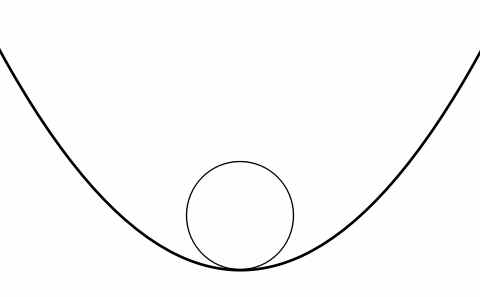
\includegraphics[width=\textwidth]{img/estabilidad1.png}
		\caption{Punto de equilibrio estable.}
		\label{fig:estabilidad1}
	\end{subfigure}
	\begin{subfigure}[b]{0.30\textwidth}
		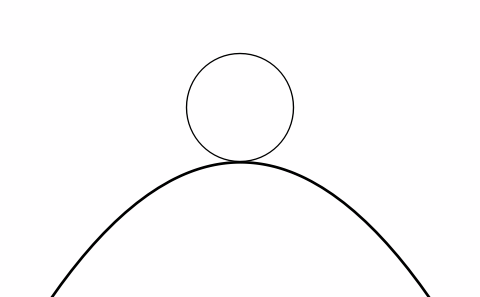
\includegraphics[width=\textwidth]{img/estabilidad2.png}
		\caption{Punto de equilibrio inestable}
		\label{fig:estabilidad2}
	\end{subfigure}
	\caption{Puntos de equilibrio.}
	\label{fig:estabilidad}
	
\end{figure}

Se dice que un sistema es BIBO (\textit{Bounded input bounded output}) estable si a entradas acotadas corresponden salidas acotadas.

Retomando el ejemplo de la figura \ref{fig:estabilidad}, si se aplica un desplazamiento hacia la derecha, en el caso \ref{fig:estabilidad1}, corresponde a una pequeña entrada a la que se le asigna una pequeña salida; por otro lado, si se le aplica una pequeña entrada al caso \ref{fig:estabilidad2}, la diferencia de la respuesta del sistema es mucho más grande \cite{dinamicos}.

\subsection{Invariante en el tiempo}

Se dice que un sistema es invariante en el tiempo si un corrimiento en el tiempo en la señal de entrada causa el mismo corrimiento en el tiempo de la señal de salida del sistema. Si $y(t)$ es la salida de un sistema cuando la entrada es $x(n)$, entonces $y(t - t_0)$ es la salida cuando se aplica la señal de entrada $x(t - t_0)$ \cite{dinamicos}.

\end{comment}

\begin{comment}
\section{Sistemas dinámicos}

Como ya se mencionó, un sistema dinámico es aquel en el cual existe un almacenamiento de energía, materia e información, es decir, es un sistema que posee memoria.



	De acuerdo con \cite{modelado_sis_det}, podemos definir a un sistema dinámico determinista de la siguiente manera.

\begin{definition}
	
	Un sistema dinámico determinista se define como una colección $D = <T, U, \Omega, Y, Q, \Delta, \varLambda>$ donde: 
	
	\begin{itemize}
		
		\item $T$ es la base del tiempo (el conjunto de valores posibles para la variable $t$).
		
		\item $U$ es el conjunto de valores posibles de la entrada.
		
		\item $\Omega$ es el conjunto de segmentos admisibles de entrada (sus elementos son funciones $\omega : [t_1, t_2] \subset T \to U$).
		
		\item $Y$ es el conjunto de valores de salida.
		
		\item $Q$ es el conjunto de valores posibles de los estados.
		
		\item $\Delta: Q \times \Omega \to Q$ es la función de transición de estados.
		
		\item $\varLambda: Q \to Y$ es la función de salida.
		
	\end{itemize}
	
\end{definition}

La función de transición $\Delta$ se caracteriza por:

\begin{itemize}
	
	\item Dado un segmento de entrada admisible $\omega: [t_1, t_2] \subset T \to U$ y sabiendo que el estado en $t_1$ es $q(t_1) \in Q$, entonces $q(t_2) = \Delta(q(t_1),\omega)$. Es decir, $\Delta$ transforma el estado inicial y la entrada en el estado final. 
	
	\item Dados dos segmentos de entrada admisibles consecutivos $\omega_1: [t_1, t_2] \to U$ y $\omega_2:[t_3, t_4] \to U$, y asumiendo que la concatenación $\omega_1 \circ \omega_2 \in \Omega$, debe cumplirse que $\Delta(q, \omega_1 \circ \omega_2) = \Delta(\Delta(q, \omega_1), \omega_2)$. Esta propiedad garantiza que la evolución del sistema sea compatible con el procesamiento secuencial de entradas.
	
\end{itemize}

\end{comment}

\section{Teoría del caos}

De acuerdo con \cite{Simon2025_caos}, el caos trata con sistemas cuyo comportamiento es impredecible a largo plazo. Suele ser asociado a sistemas aleatorios o que no tienen un orden, pero en teoría del caos se refiere a todos aquellos sistemas deterministas cuya predicción en instantes de tiempo futuro se vuelve difícil de calcular. 

Las condiciones iniciales suelen contener errores que incrementarán exponencialmente con el tiempo, lo que se conoce como sensibilidad a las condiciones iniciales, haciendo imposible la predicción a largo plazo. Estos se conocen como sistemas caóticos.

\begin{definition}
	Sea $X$ un espacio métrico y sea $\phi: X \to X$ una aplicación continua. Se dice que un sistema es caótico si cumple las siguientes condiciones:
	
	\begin{itemize}
		\item La aplicación $\phi: X \to X$ es topológicamente transitiva. 
		\item El conjunto de puntos de $\phi$ es denso en el atractor. 
		\item La aplicación $\phi: X \to X$ tiene dependencias sensitivas a las condiciones iniciales. 
	\end{itemize}	
	
\end{definition}

El hecho de que la aplicación sea topológicamente transitiva implica que el atractor caótico es irreducible, es decir, si iteramos la función $\phi$ un número determinado de veces (evolucionar el sistema durante un periodo de tiempo suficiente), se puede acceder a cualquier punto del atractor desde cualquier otro.

Si el conjunto de puntos es denso en el atractor, entonces cualquier punto en el espacio está arbitrariamente cerca de una órbita periódica. 

Finalmente, la sensibilidad a las condiciones iniciales refleja el hecho de que en un sistema caótico, dos trayectorias que inician relativamente cerca acabarán comportándose de una forma diferente a largo plazo. 

\begin{comment}
	\subsection{Exponentes de Lyapunov}

Para evaluar la sensibilidad de las condiciones se utilizan los exponentes de Lyapunov. Los cuales cuantifican la estabilidad o inestabilidad de las trayectorias en el espacio de fases al sufrir una perturbación ligera. Supongamos que tenemos dos trayectorias próximas separadas por una distancia $\delta \epsilon_0$; entonces la distancia entre ellas diverge de la forma:

\begin{equation}
	\delta_\epsilon(t) \sim \delta \epsilon_0 e^{\lambda t}
\end{equation}

Donde $\lambda$ es el exponente de Lyapunov. Es decir, mide la tasa de separación entre dos trayectorias cercanas en el espacio de fases. En un espacio de fases $n$-dimensional, existen $n$ exponentes de Lyapunov, lo que se conoce como espectro de Lyapunov. 
\end{comment}

\subsection{Atractores}

En un espacio disipado, la región del espacio de fases que atrae a las trayectorias vecinas se conoce como atractor. Es un subconjunto en el espacio de fases, es decir, un conjunto de estados a los que tiende a evolucionar el sistema en función de las condiciones iniciales.

\begin{definition}
	Sea $X$ el espacio de fases de un sistema dinámico disipado y sea $\phi_t: X \to X$ la transformación que describe el movimiento. Se dice que $A \subset X$ es un atractor si verifica las siguientes condiciones:
	
	\begin{itemize}
		
		\item $\exists U$ entorno de $A$, llamado cuenca de atracción de $A$, tal que $\forall V$ abierto con $A \subset V$, existe un $T_0$ tal que $\phi_t(U) \subset V, \forall t > T_0$.
		
		\item $\phi_t(A) = A, \forall t > 0$
		
		\item $\nexists S \subset A$ subconjunto propio no vacío que satisfaga las dos propiedades anteriores.
		
	\end{itemize} 
	
\end{definition} 

Es decir, un punto que se encuentra en el atractor no puede salir de ahí y existe una órbita alrededor de este en donde, para cualquier tiempo, la trayectoria permanece en la órbita.

\subsubsection{Tipos de atractores}

A continuación, se describen los cuatro tipos de atractores que se encuentran en la figura \ref{fig:atractores}.

\begin{enumerate}
	
	\item Atractores de punto fijo:  Un atractor es de punto fijo si existe un punto fijo tal que todas las trayectorias cercanas convergen a el cuando $t \to \infty$.

	La figura \ref{fig:punto_fijo} muestra el comportamiento de  un péndulo con resistencia al viento que responde a la ecuación:
	\begin{equation*}
		\theta'' + \gamma \theta' + \beta \theta' |\theta'| + \frac{g}{L} \sin(\theta) = 0
	\end{equation*}
	La energía se disipa por la fricción $\gamma$ y por la resistencia del aire $\beta$, obligando al sistema a perder velocidad hasta detenerse en el origen.

	\item Atractores de ciclo límite: Las trayectorias vecinas se acercan o se alejan del ciclo límite en forma de espiral. 
	
	En la figura \ref{fig:ciclo_limite} se muestra el oscilador de Van der Pol, cuya dinámica esta definida por:
	\begin{equation*}
		x'' - \mu (1 - x^2) x' + x = 0
	\end{equation*}
	El sistema aumenta la energía cuando la amplitud es pequeña y la disipa si es grande, por lo que todas las trayectorias convergen a una órbita periódica estable. 
	
	\item Atractores cuasiperiódicos: Cuando dos ciclos límites con diferentes trayectorias se superponen, estas se enroscan en las direcciones longitudinales y latitudinales, creando una figura toroidal.
	
	La Figura \ref{fig:cuasi_periodico} ilustra un oscilador lineal forzado con una frecuencia externa basada en la razón áurea $\phi$:
	\begin{equation*}
		x'' + x = A \cos(\phi t)
	\end{equation*}
	Debido a que $\phi$ es irracional respecto a la frecuencia del oscilador, el movimiento resultante es una superposición de trayectorias que nunca se repiten exactamente.
	
	\item Atractores extraños: Se dice que un atractor es extraño si tiene dimensión fractal (patrón de autosimilitud a diferentes escalas). Además, un atractor extraño es caótico si las trayectorias del sistema son atraídas hacia él, pero dentro del atractor son inestables. Esto significa que son sensibles a las condiciones iniciales.
	
	La Figura \ref{fig:caotico} muestra el atractor de Rössler, definido por el siguiente sistema de ecuaciones:
	\begin{equation*}
		\begin{cases}
			x' = -y - z \\
			y' = x + ay \\
			z' = b + z(x - c)
		\end{cases}
	\end{equation*}
	Las trayectorias se atraen hacia una estructura geométrica compleja donde se estiran y se pliegan continuamente, lo que genera un comportamiento impredecible a largo plazo a pesar de ser un sistema determinista.
\end{enumerate}

\begin{figure}[!htbp]
	\centering
	\begin{subfigure}[b]{0.40\textwidth}
		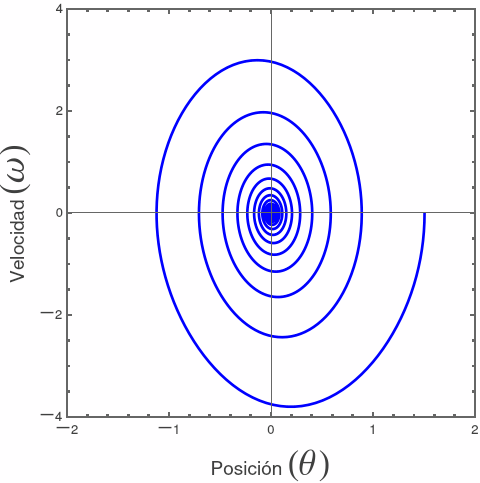
\includegraphics[width=\textwidth]{img/punto_fijo.png}
		\caption{Punto fijo: Convergencia al reposo en un péndulo amortiguado.}
		\label{fig:punto_fijo}
	\end{subfigure}
	\begin{subfigure}[b]{0.40\textwidth}
		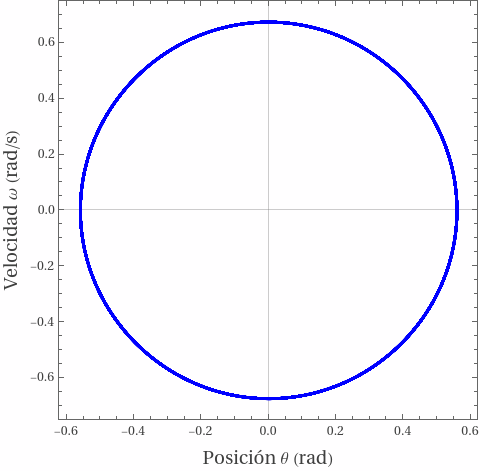
\includegraphics[width=\textwidth]{img/ciclo_limite.png}
		\caption{Ciclo límite: Oscilador de Van der Pol.}
		\label{fig:ciclo_limite}
	\end{subfigure}
	\begin{subfigure}[b]{0.40\textwidth}
		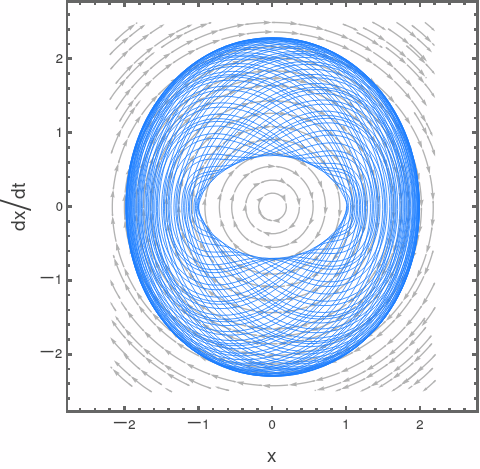
\includegraphics[width=\textwidth]{img/cuasiperiodico.png}
		\caption{Cuasiperiódico: Trayectoria densa generada por frecuencias inconmensurables.}
		\label{fig:cuasi_periodico}
	\end{subfigure}
	\begin{subfigure}[b]{0.40\textwidth}
		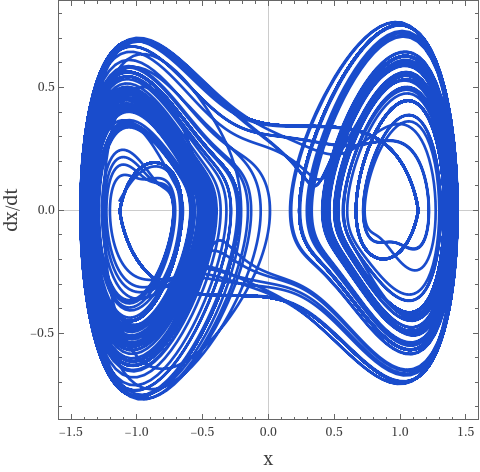
\includegraphics[width=\textwidth]{img/caotico.png}
		\caption{Extraño: Atractor de Rössler que exhibe una estructura fractal y caos.}
		\label{fig:caotico}
	\end{subfigure}
	\caption{Representación de los cuatro tipos principales de atractores en el espacio de fases.}
	\label{fig:atractores}
\end{figure}

\section{Sistemas complejos}

Los sistemas complejos son sistemas dinámicos con muchas componentes que interactúan entre sí mediante el intercambio de materia, energía o información y que, eventualmente, sufren la acción de agentes externos \cite{Torres2025_complejo}. Las colonias de hormigas, el mercado bursátil, el clima, el sistema nervioso, las células y los organismos vivos son algunos ejemplos de sistemas complejos. Estos se caracterizan por tener un conjunto de elementos que interactúan entre sí con el fin de alcanzar un objetivo \cite{Zelinka2014_cs, Zelinka2018_cs}. 

Los sistemas complejos tienen dos implicaciones fundamentales: (1) Existe una influencia mutua entre sus elementos, donde el cambio afecta inevitablemente al resto de elementos, y (2) persiguen un objetivo \cite{Zelinka2018_cs}. Además, de acuerdo con \cite{sole1996_cs_caos}, los sistemas complejos están estrechamente relacionados con la teoría del caos, pues la interacción de múltiples elementos locales puede llevar al sistema completo a lo que llama ``borde del caos'', una región donde el sistema es lo suficientemente estable para mantener su estructura, pero se mantiene flexible para generar nuevos patrones.

\begin{definition}
	Un sistema complejo es una entidad compuesta de partes interconectadas, de tal forma que el comportamiento colectivo es más que la suma de sus componentes individuales.
\end{definition}

Para entender el comportamiento de un sistema es necesario conocer los elementos y sus interacciones. Es decir, se requiere conocer los estados, valores instantáneos de todos los elementos; y sus transiciones, es decir, los cambios dinámicos en los estados.

Los sistemas complejos se caracterizan principalmente por:

\begin{itemize}
	
	\item \textbf{No linealidad}: No cumple el principio de superposición, es decir, el resultado no puede expresarse como la suma de las respuestas individuales a cada estímulo por separado. Resulta difícil predecir su evolución dinámica futura \cite{Zelinka2018_cs, Moriello2003_cs}.

	\item \textbf{Retroalimentación}: Las salidas pasadas influyen en las siguientes salidas. Este comportamiento hace alusión a la memoria del sistema \cite{Moriello2003_cs}. 
	
	\item \textbf{Orden espontáneo}: Existe un orden emergente resultado de las interacciones locales no coordinadas, el cual no puede ser descrito mediante sus interacciones locales \cite{Moriello2003_cs}.
	
	\textbf{Aparición (\textit{emergence})}: Entidades, patrones, comportamientos y propiedades emergen de la interacción de entidades más pequeñas, las cuales no exhiben estos atributos \cite{Moriello2003_cs}.

	\textbf{Elementos múltiples}: Compuesto de múltiples elementos relativamente idénticos con interacciones locales \cite{Zelinka2018_cs}. 
\end{itemize}

\section{Modelado de sistemas complejos}

Resulta evidente que predecir el comportamiento de estos sistemas es una tarea complicada. Una aproximación es el uso de modelos científicos y matemáticos, los cuales se construyen para desarrollar procesos de inferencia sobre aspectos observados en la vida real. El modelo de inferencia se realiza para entender el sistema real observado.

El proceso, de manera simplificada, se compone de tres fases, como se observa en la figura \ref{fig:cs_cientifico}:

\begin{itemize}
	
	\item Se abstrae el sistema real a un modelo, el cual puede trascender a otros sistemas reales.
	
	\item El modelo realiza un proceso de inferencia que busca averiguar las implicaciones derivadas de las premisas.
	
	\item Los resultados se utilizan para analizar, interpretar y aplicar a un sistema real. Esta aplicación no requiere ser práctica; es una relación entre las inferencias obtenidas con el modelo y el sistema real.
	
\end{itemize}

\begin{figure}[H]
	
	\centering
	
	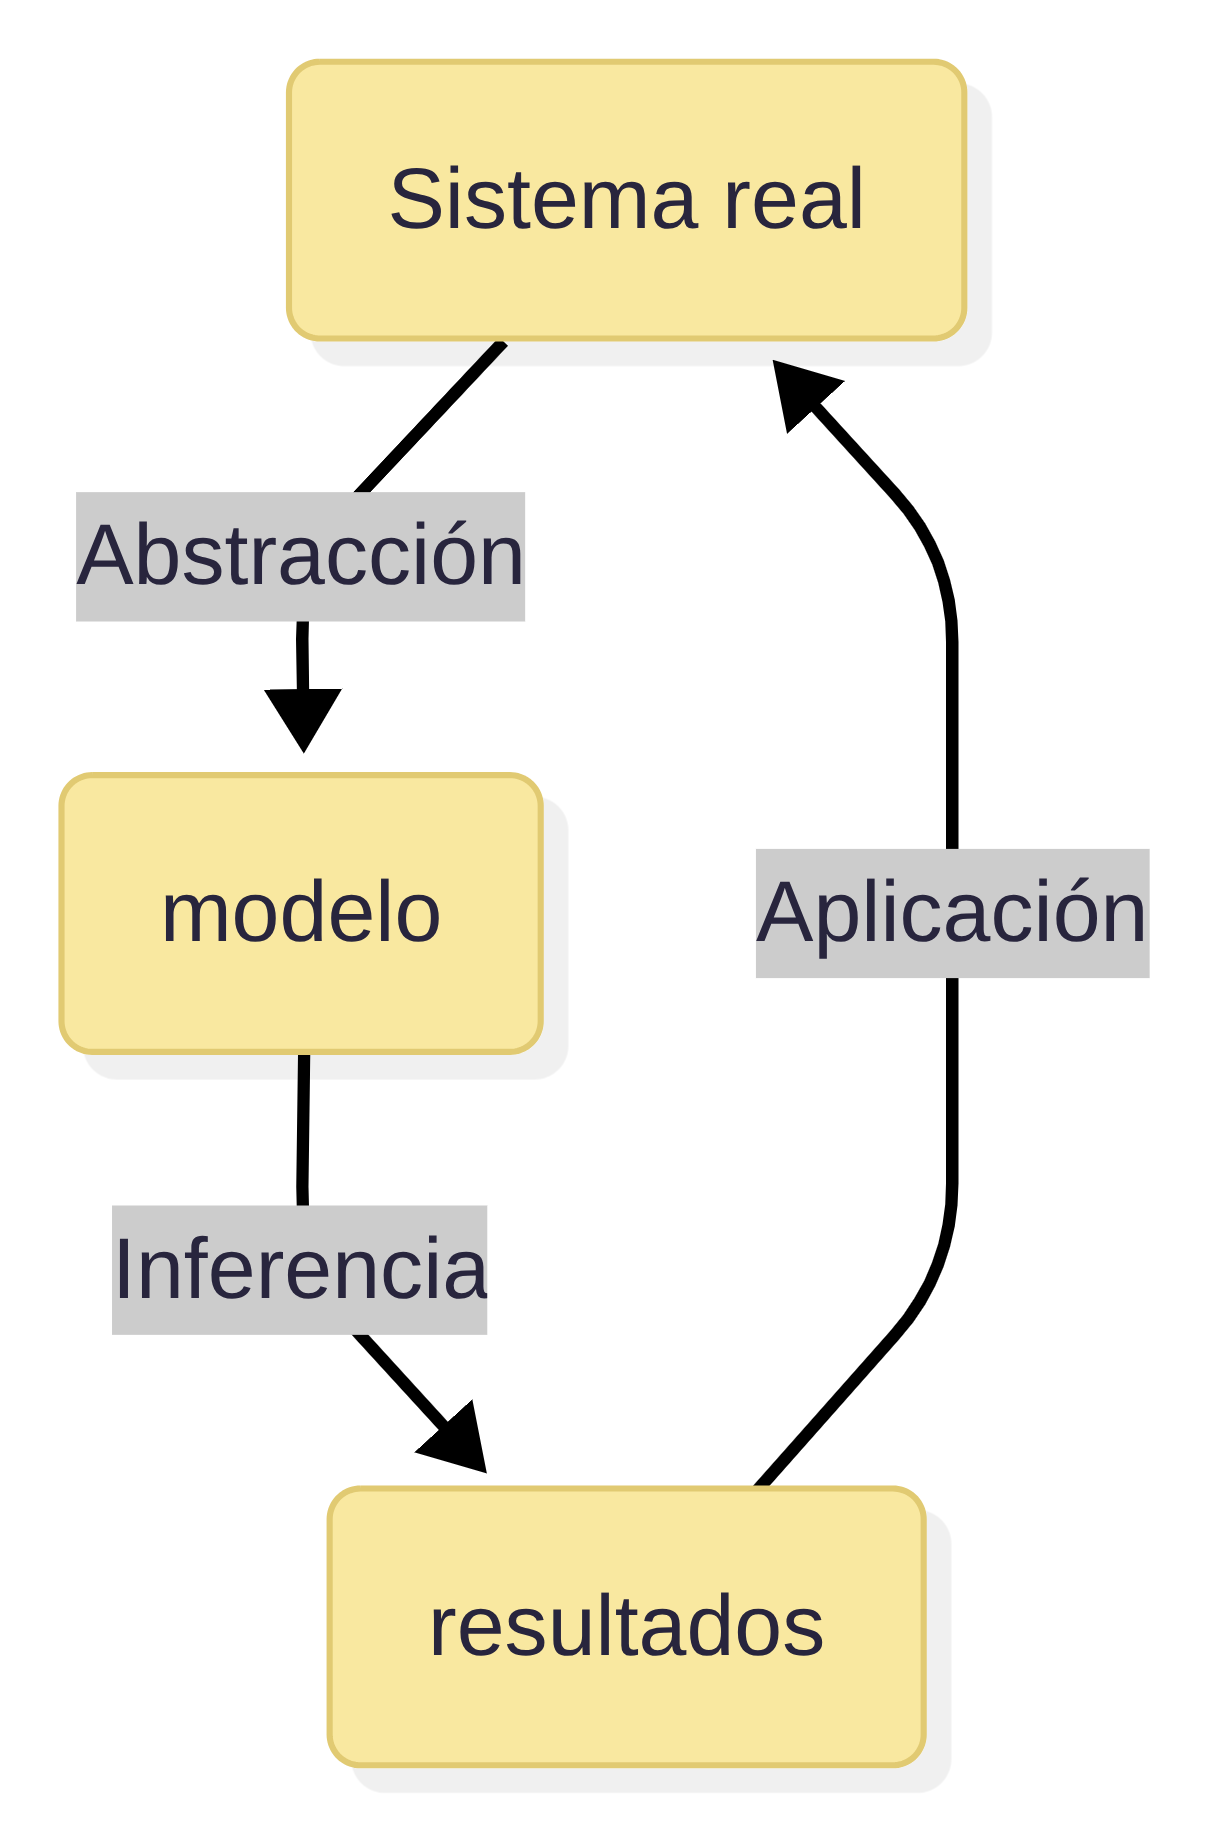
\includegraphics[width=0.3\linewidth]{img/cs_cientifico.png}
	
	\caption{Representación gráfica del modelado científico. Este proceso busca relacionar eventos del mundo real utilizando un modelo que realiza una inferencia.}
	
	\label{fig:cs_cientifico}
	
\end{figure}

%Definir que es simular

Sin embargo, estos modelos suelen carecer de las herramientas necesarias que les permiten deducir las implicaciones lógicas necesarias. Es aquí donde la computación permite agilizar este proceso realizando simulaciones.

Las computadoras permiten explorar y analizar modelos formales para resolver modelos matemáticos. Además, dado que un modelo computacional puede ser definido mediante un modelo matemático, el rol de la computación es simplificar este proceso. Dicho esto, \cite{gamco2024_simulacion} define a la simulación de la siguiente manera:

\begin{definition}
	Simulación es un proceso computacional que permite imitar el comportamiento de un sistema mediante la utilización de un modelo matemático.
\end{definition}

Los resultados de la simulación provienen del uso de reglas algorítmicas. Por eso, es necesario ampliar el proceso de abstracción y crear un modelo formal que será utilizado por la computadora, como se muestra en la figura \ref{fig:cs_computacional}.

\begin{figure}[H]
	
	\centering
	
	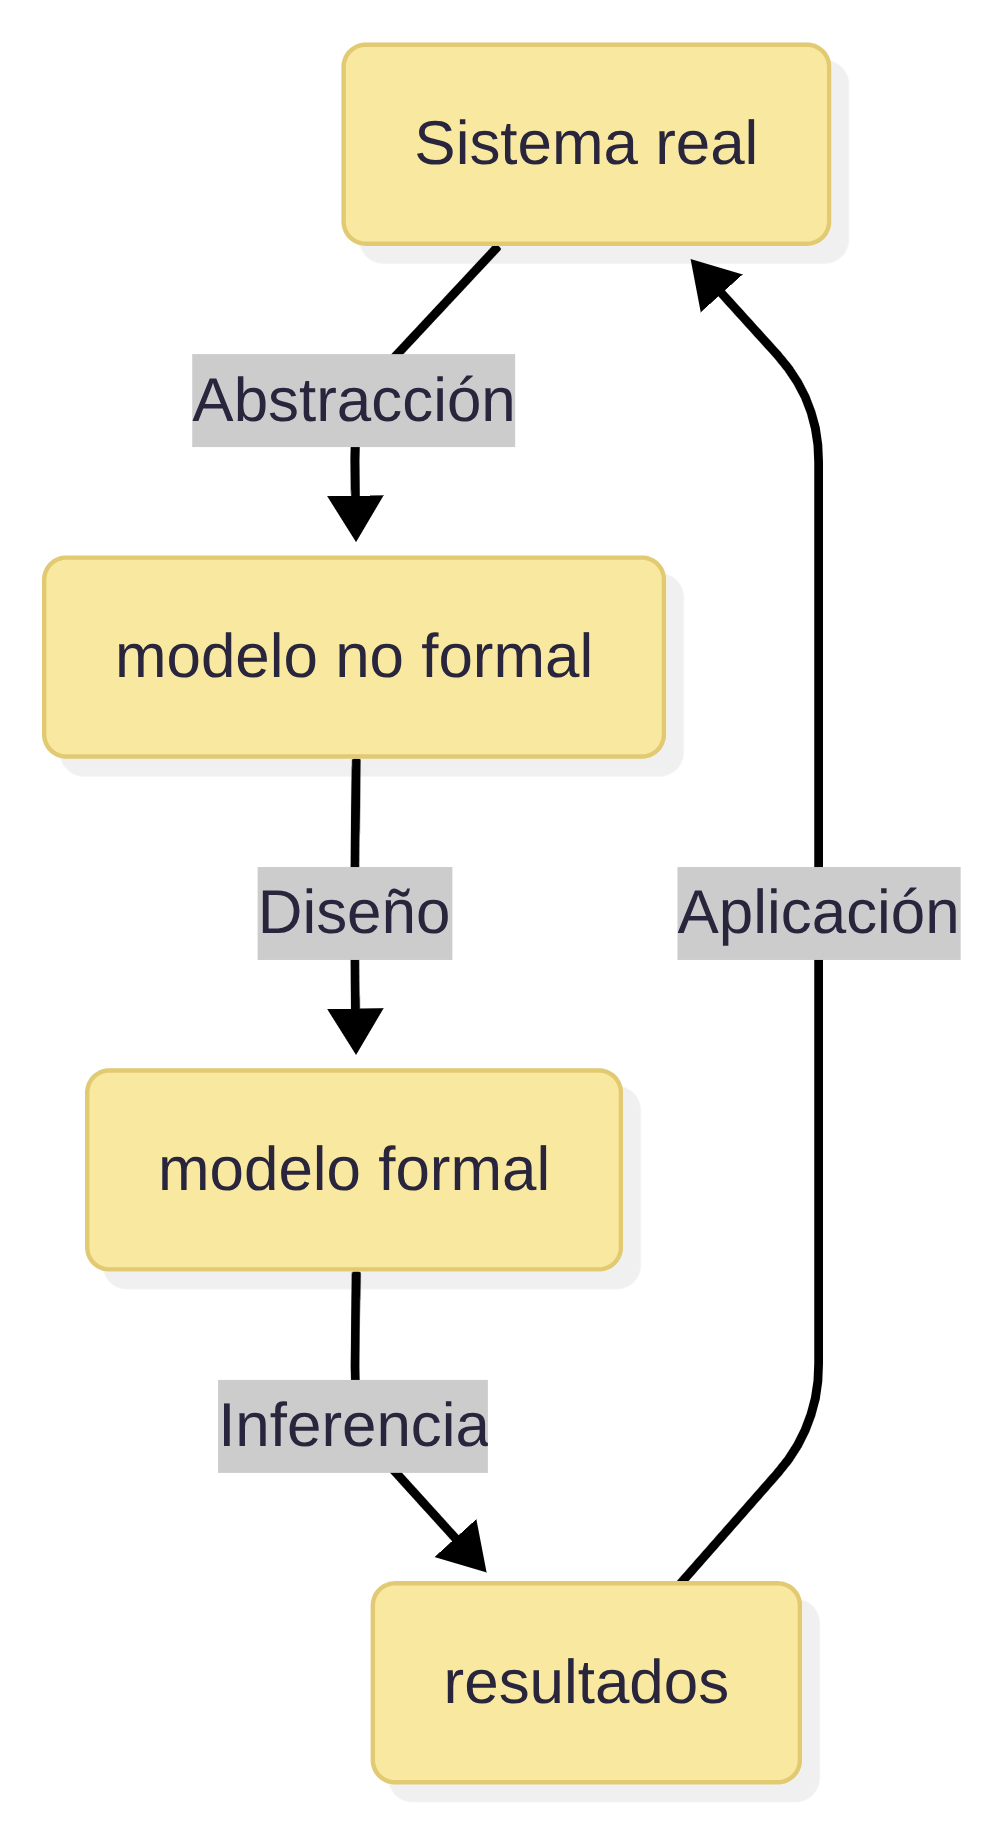
\includegraphics[width=0.3\linewidth]{img/cs_computacional.png}
	
	\caption{Representación gráfica del modelado computacional. Relaciona eventos del mundo real utilizando un modelo computacional que ayuda a agilizar el proceso de inferencia.}
	
	\label{fig:cs_computacional}
	
\end{figure}

Se requiere de un experto en el sistema real que pueda abstraer el problema y un modelador que formalice dicha abstracción para ejecutarla en una computadora que infiera los resultados, mismos que utilizará nuevamente el experto en el sistema real para entablar la relación con el sistema real \cite{Izquierdo2008_modelado}.

Para estudiar sistemas complejos hay varias herramientas de simulación. Una de ellas son los autómatas celulares \cite{Torres2025_complejo, sole1996_cs_caos, Hoekstra2010_cs_ca}, los cuales siguen la caracterización de los sistemas complejos: elementos idénticos con interacciones locales que pueden generar orden espontáneo, comportamientos emergentes e incluso retroalimentados. 
\clearpage